
\subsubsection{Module MD-11: Quản lý Quan hệ Khách hàng (CRM)}
Module Quản lý Quan hệ Khách hàng (MD-11) là một công cụ chiến lược giúp nhà hàng xây dựng và duy trì mối quan hệ bền chặt với khách hàng. Module này tập trung vào việc thu thập, lưu trữ, quản lý thông tin khách hàng, theo dõi lịch sử tương tác, phân loại khách hàng, quản lý các chương trình khuyến mãi/voucher, và thu thập phản hồi/đánh giá từ khách hàng. Mục tiêu cuối cùng là nâng cao sự hài lòng của khách hàng, tăng cường lòng trung thành và thúc đẩy doanh thu.



\begin{figure}[H]
    \centering
    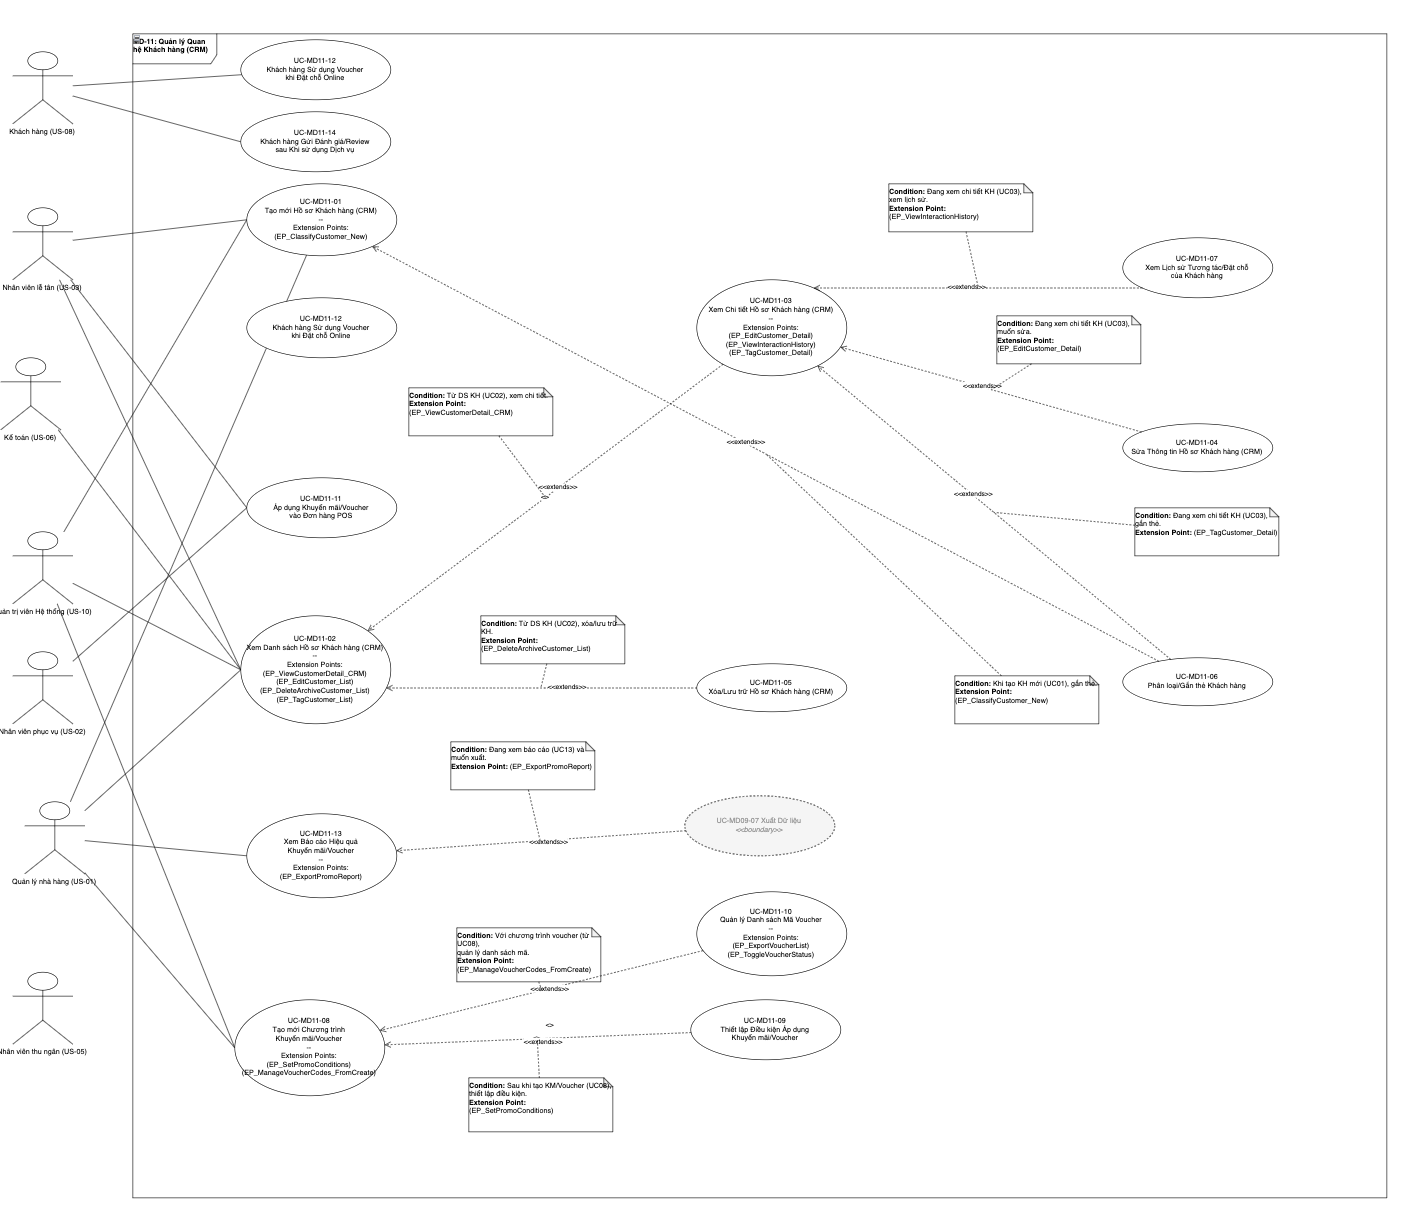
\includegraphics[width=15cm]{Sections/tong_quan/functional_spec/img/uc11.png}
    \vspace{0.5cm}
    \caption{Use case diagram cho Module MD-11}
    \label{fig:my_label}
\end{figure}

\begin{longtable}{|m{2cm}|m{2.5cm}|m{2.5cm}|m{4.5cm}|m{4cm}|}
\caption{Danh sách Yêu cầu Chức năng cho Module MD-11: Quản lý Quan hệ Khách hàng (CRM)} \label{tab:fr_md11_crm_marketing_revised_in_codeblock} \\
\hline
\textbf{Mã Module} & \textbf{Mã Yêu cầu CN} & \textbf{Mã Người dùng} & \textbf{Tên Chức năng} & \textbf{Mô tả Ngắn} \\
\hline
\endhead % Header cho các trang tiếp theo
\midrule
\endfoot % Footer cho bảng
\bottomrule
\endlastfoot % Footer cho trang cuối cùng

% === Quản lý Hồ sơ Khách hàng (CRM View) - Tách nhỏ ===
MD-11 & FR-MD11-01 & US-01, US-03, US-10 & Tạo mới Hồ sơ Khách hàng (CRM) & Nhân viên/Quản lý tạo hồ sơ mới cho khách hàng với các thông tin chi tiết. \\
\hline
MD-11 & FR-MD11-02 & US-01, US-03, US-10 & Xem Danh sách Hồ sơ Khách hàng (CRM) & Xem danh sách tất cả khách hàng trong hệ thống CRM, có thể tìm kiếm, lọc. \\
\hline
MD-11 & FR-MD11-03 & US-01, US-03, US-10 & Xem Chi tiết Hồ sơ Khách hàng (CRM) & Xem toàn bộ thông tin chi tiết của một khách hàng cụ thể (thông tin cá nhân, lịch sử, sở thích...). \\
\hline
MD-11 & FR-MD11-04 & US-01, US-03, US-10 & Sửa Thông tin Hồ sơ Khách hàng (CRM) & Cập nhật, chỉnh sửa các thông tin trong hồ sơ của một khách hàng đã có. \\
\hline
MD-11 & FR-MD11-05 & US-01, US-10 & Xóa/Lưu trữ Hồ sơ Khách hàng (CRM) & Xóa (nếu chưa có giao dịch) hoặc lưu trữ (ẩn đi) hồ sơ khách hàng không còn hoạt động. \\
\hline
MD-11 & FR-MD11-06 & US-01, US-06, US-10 & Phân loại/Gắn thẻ Khách hàng & Phân loại khách hàng (VIP, thường xuyên...) hoặc gắn thẻ (tag) cho khách hàng để phục vụ marketing, chăm sóc. \\
\hline
MD-11 & FR-MD11-07 & US-01, US-06, US-10 & Xem Lịch sử Tương tác/Đặt chỗ của Khách hàng & Truy cập toàn bộ lịch sử đặt chỗ, hóa đơn, phản hồi, ghi chú tương tác của một khách hàng cụ thể. \\
\hline

% === Quản lý Voucher/Khuyến mãi ===
MD-11 & FR-MD11-08 & US-01, US-10 & Tạo mới Chương trình Khuyến mãi/Voucher & Định nghĩa các chương trình khuyến mãi (giảm giá \%, giảm tiền cố định, mua X tặng Y) hoặc tạo mã voucher. \\
\hline
MD-11 & FR-MD11-09 & US-01, US-10 & Thiết lập Điều kiện Áp dụng Khuyến mãi/Voucher & Cấu hình điều kiện: thời gian, giá trị đơn tối thiểu, sản phẩm/danh mục áp dụng, số lần sử dụng... \\
\hline
MD-11 & FR-MD11-10 & US-01, US-10 & Quản lý Danh sách Mã Voucher & Xem danh sách mã voucher đã tạo, trạng thái (đã dùng, còn hạn), có thể xuất mã hàng loạt, vô hiệu hóa voucher. \\
\hline
MD-11 & FR-MD11-11 & US-02, US-05 & Áp dụng Khuyến mãi/Voucher vào Đơn hàng POS & Nhân viên POS nhập mã voucher hoặc chọn chương trình khuyến mãi đủ điều kiện để áp dụng cho đơn hàng. \\
\hline
MD-11 & FR-MD11-12 & US-08 & Khách hàng Sử dụng Voucher khi Đặt chỗ Online & Khách hàng nhập mã voucher hợp lệ vào đơn đặt chỗ/đặt món online để được giảm giá. \\
\hline
MD-11 & FR-MD11-13 & US-01 & Xem Báo cáo Hiệu quả Khuyến mãi/Voucher & Thống kê số lần sử dụng, tổng giá trị giảm giá của từng chương trình/voucher. (Mở rộng từ UC-MD09-09) \\
\hline

% === Thu thập & Quản lý Đánh giá/Phản hồi ===
MD-11 & FR-MD11-14 & US-08 & Khách hàng Gửi Đánh giá/Review sau Khi sử dụng Dịch vụ & Khách hàng (có thể qua email mời hoặc link trên hóa đơn) gửi đánh giá về chất lượng món ăn, dịch vụ. \\
\hline
MD-11 & FR-MD11-15 & US-01, US-09 & Xem và Quản lý Đánh giá/Phản hồi của Khách hàng & Quản lý xem các đánh giá, có thể phản hồi, phân loại (tích cực, tiêu cực), hoặc đánh dấu đã xử lý. \\
\hline
MD-11 & FR-MD11-16 & US-01 & (Tùy chọn) Hiển thị Đánh giá Tích cực trên Website & Chọn lọc và hiển thị các đánh giá tốt của khách hàng trên trang web nhà hàng (nếu muốn). \\
\hline
% Các chức năng khác như Loyalty, Email Marketing sẽ được thêm vào sau nếu cần
\end{longtable}

\subsubsubsection{Mục tiêu và Phạm vi}
\label{sssec:md11_objectives_scope}
Mục tiêu chính của module MD-11 là:
\begin{itemize}
    \item \textbf{Xây dựng cơ sở dữ liệu khách hàng toàn diện:} Lưu trữ thông tin liên hệ, lịch sử giao dịch, sở thích và các ghi chú quan trọng về từng khách hàng.
    \item \textbf{Phân loại và phân khúc khách hàng:} Cho phép gắn thẻ, phân loại khách hàng (ví dụ: VIP, khách thường xuyên) để phục vụ các chiến dịch chăm sóc và marketing cá nhân hóa.
    \item \textbf{Quản lý chương trình khuyến mãi và voucher hiệu quả:} Tạo, cấu hình điều kiện áp dụng, theo dõi việc sử dụng và đánh giá hiệu quả của các chương trình khuyến mãi và mã voucher.
    \item \textbf{Thu thập và quản lý phản hồi của khách hàng:} Cung cấp kênh cho khách hàng gửi đánh giá và cho phép nhà hàng xem xét, phân tích các phản hồi này.
    \item \textbf{Tăng cường tương tác và chăm sóc khách hàng:} Cung cấp thông tin để nhân viên có thể phục vụ khách hàng tốt hơn và xây dựng mối quan hệ lâu dài.
    \item \textbf{Hỗ trợ các hoạt động marketing:} Cung cấp dữ liệu khách hàng cho việc tạo các chiến dịch email marketing hoặc các hoạt động quảng bá khác (có thể tích hợp với module marketing riêng).
\end{itemize}
Phạm vi của module bao gồm việc quản lý hồ sơ khách hàng từ khi tạo mới, cập nhật thông tin, theo dõi lịch sử, cho đến việc thiết kế và quản lý các chương trình khuyến mãi/voucher, cũng như quy trình thu thập và xem xét đánh giá từ khách hàng.

\subsubsubsection{Đối tượng Sử dụng Chính}
\label{sssec:md11_primary_users}
Các đối tượng người dùng chính tương tác với module này bao gồm:
\begin{itemize}
    \item \textbf{US-01 (Quản lý nhà hàng):} Là người dùng chính, chịu trách nhiệm tạo và quản lý các chương trình khuyến mãi, xem báo cáo hiệu quả, quản lý hồ sơ khách hàng VIP, và xem xét các đánh giá của khách hàng.
    \item \textbf{US-03 (Nhân viên lễ tân):} Thường xuyên tạo mới và cập nhật hồ sơ khách hàng, có thể xem lịch sử đặt chỗ của khách để hỗ trợ tốt hơn.
    \item \textbf{US-06 (Kế toán):} Có thể cần xem thông tin khách hàng liên quan đến hóa đơn hoặc các chương trình khách hàng thân thiết.
    \item \textbf{US-10 (Quản trị viên Hệ thống):} Có thể tham gia vào việc cấu hình ban đầu của module CRM, tạo các trường tùy chỉnh hoặc thiết lập các quy tắc tự động (nếu có).
    \item \textbf{US-08 (Khách hàng):} Là người cung cấp thông tin cá nhân, sử dụng voucher khi đặt chỗ online, và gửi đánh giá/review về dịch vụ.
    \item \textbf{US-02 (Nhân viên phục vụ) / US-05 (Nhân viên thu ngân):} Áp dụng các chương trình khuyến mãi hoặc mã voucher cho đơn hàng tại POS.
\end{itemize}

\subsubsubsection{Các Chức năng Chính}
\label{sssec:md11_key_functionalities}
Module MD-11 cung cấp một bộ các chức năng tập trung vào việc quản lý và tăng cường mối quan hệ với khách hàng:

\begin{itemize}
    \item \textbf{Quản lý Hồ sơ Khách hàng (UC-MD11-01 đến UC-MD11-07):}
    \begin{itemize}
        \item Tạo mới một hồ sơ khách hàng trong hệ thống CRM với các thông tin liên hệ cơ bản (UC-MD11-01).
        \item Xem danh sách tất cả các hồ sơ khách hàng với khả năng tìm kiếm và lọc (UC-MD11-02).
        \item Xem thông tin chi tiết đầy đủ của một hồ sơ khách hàng, bao gồm lịch sử giao dịch và tương tác (UC-MD11-03).
        \item Sửa đổi và cập nhật các thông tin trong một hồ sơ khách hàng đã tồn tại (UC-MD11-04).
        \item Xóa vĩnh viễn (nếu không có giao dịch) hoặc lưu trữ (ẩn đi) các hồ sơ khách hàng không còn phù hợp (UC-MD11-05).
        \item Gán các thẻ (tags) hoặc phân loại khách hàng (ví dụ: VIP, Thường xuyên) để phục vụ việc nhóm và phân tích (UC-MD11-06).
        \item Truy cập và xem lại toàn bộ lịch sử các hoạt động và giao dịch liên quan đến một khách hàng cụ thể (UC-MD11-07).
    \end{itemize}

    \item \textbf{Quản lý Chương trình Khuyến mãi và Voucher (UC-MD11-08 đến UC-MD11-13):}
    \begin{itemize}
        \item Định nghĩa một chương trình khuyến mãi mới hoặc một lô mã voucher mới, bao gồm loại hình và giá trị khuyến mãi (UC-MD11-08).
        \item Thiết lập các điều kiện và quy tắc chi tiết để chương trình/voucher có thể được áp dụng (ví dụ: thời gian hiệu lực, giá trị đơn hàng tối thiểu, sản phẩm áp dụng) (UC-MD11-09).
        \item Xem danh sách các mã voucher đã tạo, kiểm tra trạng thái, và có thể thực hiện xuất file hoặc vô hiệu hóa mã (UC-MD11-10).
        \item Nhân viên tại POS áp dụng một chương trình khuyến mãi hoặc nhập mã voucher hợp lệ vào đơn hàng của khách (UC-MD11-11).
        \item Khách hàng tự nhập và sử dụng mã voucher hợp lệ khi thực hiện đặt chỗ hoặc đặt món trước trực tuyến (UC-MD11-12).
        \item Xem báo cáo thống kê chi tiết về tình hình sử dụng và hiệu quả của các chương trình khuyến mãi hoặc voucher (UC-MD11-13).
    \end{itemize}

    \item \textbf{Quản lý Đánh giá và Phản hồi từ Khách hàng (UC-MD11-14, và sẽ có các UC tiếp theo như UC-MD11-15, UC-MD11-16):}
    \begin{itemize}
        \item Cho phép khách hàng gửi các ý kiến đánh giá, nhận xét, hoặc xếp hạng về dịch vụ của nhà hàng thông qua các kênh trực tuyến (UC-MD11-14).
        \item (Dự kiến) Cho phép Quản lý nhà hàng xem danh sách các đánh giá đã nhận được.
        \item (Dự kiến) Cho phép Quản lý nhà hàng xem chi tiết một đánh giá cụ thể và có thể thực hiện các hành động phản hồi.
    \end{itemize}
\end{itemize}

\subsubsubsection{Tóm tắt Luồng Hoạt động Tổng thể}
\label{sssec:md11_overall_workflow}
Luồng hoạt động trong module Quản lý Quan hệ Khách hàng (CRM) thường bao gồm các giai đoạn và quy trình sau:
\begin{enumerate}
    \item \textbf{Thu thập và Quản lý Thông tin Khách hàng:}
        \begin{itemize}
            \item Nhân viên Tạo mới Hồ sơ Khách hàng (CRM) (UC-MD11-01) khi có khách mới hoặc nhập dữ liệu.
            \item Nhân viên thường xuyên Xem Danh sách Hồ sơ Khách hàng (UC-MD11-02), Xem Chi tiết Hồ sơ Khách hàng (UC-MD11-03) để tra cứu, và Sửa Thông tin Hồ sơ Khách hàng (UC-MD11-04) khi cần cập nhật.
            \item Thực hiện Phân loại/Gắn thẻ Khách hàng (UC-MD11-06) để phục vụ các mục đích khác nhau.
            \item Khi cần, Xóa/Lưu trữ Hồ sơ Khách hàng (CRM) (UC-MD11-05).
            \item Xem Lịch sử Tương tác/Đặt chỗ của Khách hàng (UC-MD11-07) để hiểu rõ hơn về khách.
        \end{itemize}
    \item \textbf{Triển khai và Quản lý Chương trình Khuyến mãi/Voucher:}
        \begin{itemize}
            \item Quản lý Tạo mới Chương trình Khuyến mãi/Voucher (UC-MD11-08).
            \item Thiết lập Điều kiện Áp dụng Khuyến mãi/Voucher (UC-MD11-09) chi tiết cho từng chương trình.
            \item (Nếu là voucher) Quản lý Danh sách Mã Voucher (UC-MD11-10), có thể xuất file hoặc vô hiệu hóa mã.
            \item Nhân viên tại POS Áp dụng Khuyến mãi/Voucher vào Đơn hàng POS (UC-MD11-11) cho khách.
            \item Khách hàng Sử dụng Voucher khi Đặt chỗ Online (UC-MD11-12) trên website/app.
            \item Quản lý định kỳ Xem Báo cáo Hiệu quả Khuyến mãi/Voucher (UC-MD11-13) để đánh giá.
        \end{itemize}
    \item \textbf{Thu thập và Xử lý Phản hồi Khách hàng:}
        \begin{itemize}
            \item Khách hàng Gửi Đánh giá/Review sau Khi sử dụng Dịch vụ (UC-MD11-14).
            \item (Dự kiến) Quản lý xem xét các đánh giá này và có thể phản hồi hoặc thực hiện các hành động cải thiện dịch vụ.
        \end{itemize}
\end{enumerate}
Module MD-11 giúp nhà hàng không chỉ quản lý giao dịch mà còn xây dựng mối quan hệ ý nghĩa với khách hàng, từ đó tạo lợi thế cạnh tranh và phát triển bền vững.

